\documentclass[10pt,a4paper,report]{article}
\usepackage[utf8]{inputenc}
\usepackage[english]{babel}
\usepackage{amsmath}
\usepackage{amsfonts}
\usepackage{amssymb}
\usepackage{graphicx}
\usepackage{lmodern}
\usepackage{multirow}

\author{ Gerardo Tibamoso and Rub\'en Dorado\\ \\
	Data Mining Course, Sylvie Ratt\'e\\ \'Ecole de technologie superieure (ÉTS)}

%\title{Estimacion automatica de la trayectoria de un vaso en secuencias de ecografia abdominal}
\title{Automatic vessel tracking in abdominal ultrasound sequences}

\date{}
\begin{document}
\maketitle

%\abstract{
%El movimiento de organos abdominales durante la respiracion es importante para diagnostico y procedimientos medicos de alta precision. 
%Observaciones de este comportamiento dinamico son realizadas con frecuencia por medio de ultrasonido, por el bajo riesgo para el paciente y la generacion de imagenes en tiempo real.
%%El uso de ecografias para esta estimacion es frecuente en la practica clinica, por su bajo riesgo para el paciente, y la visualizacion imagenes en tiempo real. 
%Se propone un metodo para estimar el movimiento de un vaso en secuencias de ecografia abdominal durante respiracion normal.
%Se busca definir una funcion periodica que describa la trayectoria del vaso, basada en correlaciones entre regiones de imagenes consecutivas, empleando algoritmos de procesamiento de imagenes, técnicas estadisticas, y algoritmos de mineria de datos. 
%El metodo esta basado en correlaciones entre regiones de imagenes consecutivas, 
%para definir una funcion periodica que describa la trayectoria del vaso.
% se realiza la estimacion de una funcion periodica que describe la trayectoria del vaso.
%Se cuenta con un dataset para la experimentacion y validacion provisto por el CLUST 2015.}

\abstract{
%The abdominal organs movement during respiration is important for diagnostic and high precision medical procedures. Observations of this dynamic behavior are frequently performed  by ultrasound, due its low risk to the patient and image generation in real time. We propose an automatic vessel tracking method in abdominal ultrasound sequences during normal respiration. The method is based on correlations between regions of consecutive images, to estimate the parameters of a periodic function describing the vessel motion. Sequences of the CLUST 2015 dataset of 2D+t real ultrasound images are employed for experimentation and validation.

The observation of abdominal organs movement during respiration is
important for diagnostic and high precision medical procedures. Analysis
of this dynamic behavior are frequently performed by ultrasound, due its
low risk to the patient and image generation in real time. We propose
an automatic vessel tracking method in abdominal ultrasound sequences
during normal respiration. 
The method is based on 
image processing techniques and data modeling
to estimate the parameters of a periodic
function describing the vessel motion. Sequences of the CLUST 2015
dataset of 2D+t real ultrasound images are employed for experimentation
and validation.
}

\section{Introduction}

%La estimacion del movimiento interno en el abdomen y torax es un factor importante para diagnostico o precision de procedimientos medicos como puncion y radioterapia.Imagenes de resonancia magnetica y de ultrasonido han sido empleadas para observar y analizar estos movimientos en organos como el higado y el corazon. Sin embargo, una descripción cuantitativa y automatica de su comportamiento dinamico es un problema que aun permanece abierto. El principal desafio consiste en identificar las fronteras de las estructuras anatomicas en las imagenes, que se hacen borrosas por variaciones de intensidad y ruido generado en el proceso de la adquisicion.

The internal motion of abdomen and thorax is an important parameter to diagnosis and medical procedures as puncture and radiotherapy. Magnetic resonance imaging and ultrasound have been employed to observe these movements in organs as liver and heart. However, a quantitative description of this dynamic behavior is still an open problem \cite{Wu2016, DeLuca2013, Martinez2011}. The boundaries identification of the anatomical structures is one of the main obstacles because these are blurred due motion.

%Wu et al. \cite{Wu2016} proponen la generacion automatica de clusters de imagenes para asociarlos a las diferentes fases del ciclo respiratorio. De esta manera se identifica el efecto del movimiento de la respiracion para cada grupo de imagenes, que puede ser corregido. Sin embargo, en este documento no se describe el tipo de caracteristicas (como intensidades o bordes) que definen a los puntos que fueron extraidos y seguidos en la secuencia de imagenes.  


%De Luca et al. \cite{DeLuca2013} proponen identificar y seguir vasos sanguineos del abdomen en imagenes de ultrasonido de manera automatica, basados en informacion de intensidades y forma. El procesamiento es local, centrado en la posicion del vaso, y en su vecindad para el analisis de las imagenes consecutivas. Adicionalmente, emplea un metodo de aprendizaje basado en la periodicidad del movimiento generado por la respiracion, para inferir cuando la informacion extraida de las imagenes es incompleta. El documento no describe como son extraidas las caracteristicas de forma.

%Martinez et al. \cite{Martinez2011} se enfocan en la extraccion automatica de patrones de movimiento del corazon en imagenes de cine resonancia magnetica. Inicialmente se extraen campos vectoriales de movimiento entre frames consecutivos, como base para establecer regiones espacialmente conectadas, y realizar analisis estadistico para estimar las regiones de menor y mayor movimiento. La estimacion del campo vectorial esta basado en la informacion de bordes de las imagenes. Sin embargo, la sintonizacion del metodo es engorrosa debido a la cantidad de variables empleadas.

%Nuestra propuesta consiste en encontrar los parametros de una funcion matematica que describa la trayectoria de un punto debido al movimiento generado por la respiracion, en una secuencia de imagenes de ultrasonido de abdomen registradas desde una posicion estable sobre el cuerpo del paciente. El documento se organiza como sigue: En la seccion \ref{sec:methodology} se describe la metodologia, los resultados preliminares en la seccion \ref{sec:results}, y finalmente la discusion en la seccion \ref{sec:discussion}.

We propose to estimate the parameters of a periodic function to fit it to the trajectory of a vessel in ultrasound  sequences during normal respiration. This document is organized as follow: in section \ref{sec:methodology} the methodology is described, the preliminary results in the section \ref{sec:results}, and finally the discussion in the section \ref{sec:discussion}.


\section{Methodology}
\label{sec:methodology}

%Asumiendo que el movimiento generado por la respiracion es periodico y sin perturbaciones, este puede expresarse por una serie de Fourier,  tal que

Assuming that respiration motion has a periodic behavior and without disturbances, it can be expressed as a Fourier series, such that
\begin{equation}
F(t) = \frac{A_0}{2} + \sum_{n=1}^{N} A_n sin( 2 \pi f n  t + \phi_n )
\end{equation}
%siendo $f$ la frecuencia respiratoria, $t$ el tiempo, $A_n$ una constante que define la amplitud para cada armonico $n$, y $A_0$ y $\phi_n$ constantes que definen translaciones de la se\~nal en amplitud y tiempo, respectivamente. 

where $f$ is the respiratory frequency ($Hz$), $t$ the time, $A_n$ is the amplitude of the $n$ harmonic, and $A_0$ and $\phi_n$ are translations in amplitude and time of the signal, respectively.
%Nuestro objetivo consiste en encontrar el primer armonico de esta se\~nal que permita describir, como una primera aproximacion, el movimiento del centro de un vaso en una secuencia de imagenes abdominales de ultrasonido, como se describe en la Figura \ref{fig:pointTrajectory}.
%%%%%%%%%%%%%%%%%%%%%%%%%%%%%%%
%%%%%%%%%%%%%
With this hypothesis, the estimate of the first harmonic of $ F ( t) $ is performed . This describes the position of the blood vessel $P_v $, which moves as a result of breathing in image sequences ultrasound abdomen, as illustrated in Figure \ref{fig:pointTrajectory}.
%CCCCCCCCCCCCCCCCCon esta hipotesis se realizó la estimacion del primer armonico de $F(t)$, para describir la posicion de un vaso sanguineo $P_v$, que se mueve por efecto de la respiracion en secuencias de imagenes de ultrasonido de abdomen, como se ilustra en la Figura \ref{fig:pointTrajectory}. 
%
\begin{figure}[h!]
\centering
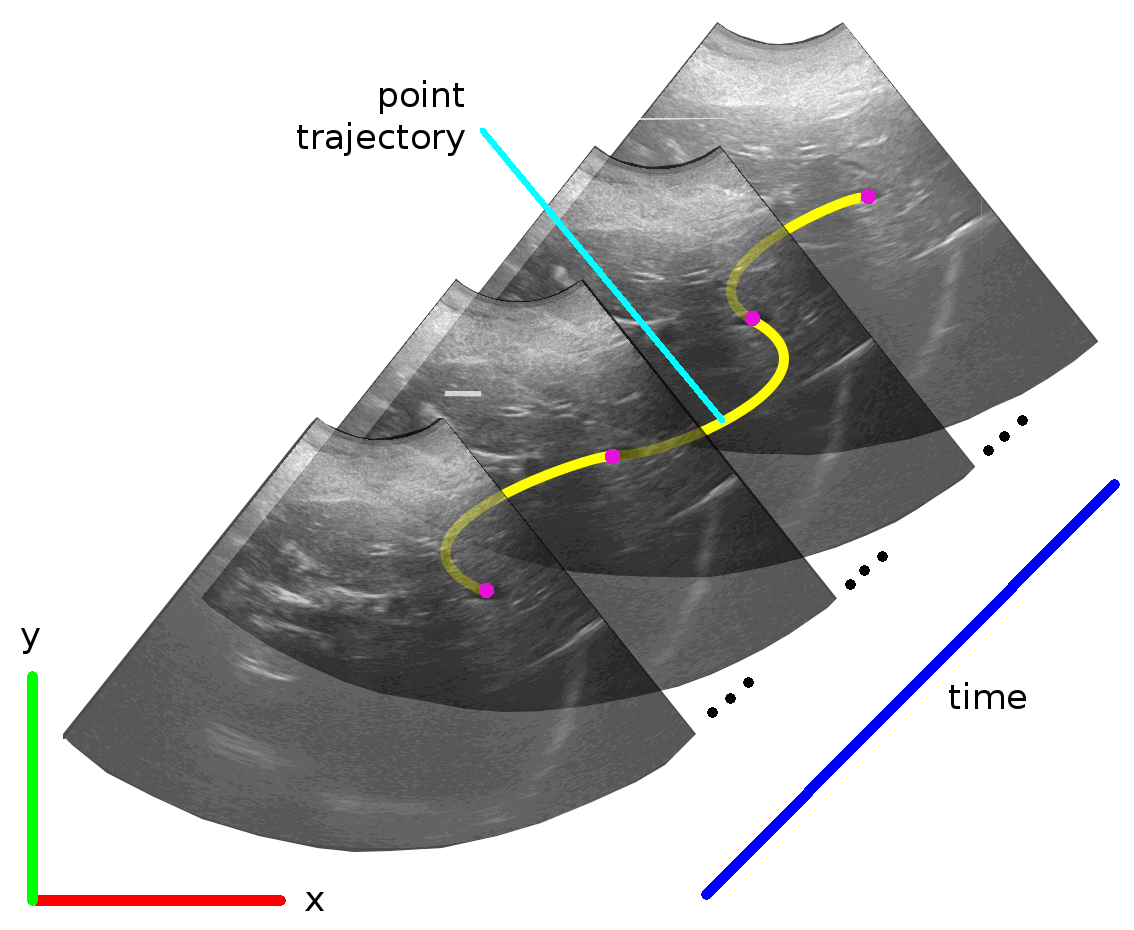
\includegraphics[width=0.6\textwidth]{figures/pointTrajectory}
\caption{2D abdominal ultrasound sequence. During the acquisition,  the position of the probe is fixed and the patient breathing is normal. In this picture is depicted an approximation of the vessel motion vs time.}
\label{fig:pointTrajectory}
\end{figure}
%
The $P_v(x,y)$ components, can be expressed as
%Las coordenadas de $P_v(x,y)$ en cada imagen $k$ ($k = 1, 2, ..., K$) de la secuencia de $K$ imagenes, se pueden expresar como
\begin{equation}
\begin{tabular}{l}
$x(k) = a_0 + a_1 sin (a_2 k + a_3)$\\
$y(k) = b_0 + b_1 sin (b_2 k + b_3)$,
\end{tabular}
\label{eq:coord}
\end{equation}
where $k$ is the number of the image in the sequence.
%siendo $k$ el numero la imagen en la secuencia. 
The parameters of $x(k)$ and $y(k)$ are estimated by means of an optimization process, where the input data are the position of the vessel obtained with image processing techniques, as illustrated in Figure \ref{fig:methodology}.
%El valor de los parametros de las funciones $x(k)$ y $y(k)$ son estimados por medio de un proceso de optimización de los datos de posicion del vaso obtenidos aplicando técnicas de procesamiento de imagenes, como se ilustra en la Figura \ref{fig:methodology}. 
%
\begin{figure}[h!]
\centering
\includegraphics[width=1.0\textwidth]{figures/methodology}
\caption{Diagram of the proposed method.}
\label{fig:methodology}
\end{figure}
%
The first step consisted in binarizing the images, to differentiate the inside from the outside of the vessel. This was done by applying thresholding on all images. The threshold was defined by an analysis of the first image histogram. Afterward, an opening morphological operation (first erosion, then dilation) was applied to remove noise and soften regions contours.
%El primer paso consistio en binarizar las imagenes, para diferenciar el interior del exterior del vaso. Esta binarizacion se realizo aplicando umbralizacion a todas las imagenes, cuyos umbral se definio por medio de un analisis del histograma de la primera imagen. Posteriormente se aplico la operacion morfologica de apertura (primero erosion, luego dilatacion), para remover ruido y suavizar los contornos de las regiones. 


The second step estimates the central position of the vessel in the binary images, from a known point of the first image (annotation expert). This starting point is used as a seed to extract a region of pixels interconnected with the same intensity. The center of this region is the center of its bounding box of minimum area (oriented with the object). This center represents the position of the vessel. To find the center in the next image the process is repeated . In this case, the seed point is sought in the new image within the previous seed and center coordinates. If the seed point fails to find a vessel internal region, the center of that image is defined as the center of the previous image, until a new seed point will be found. An additional restriction is established. The center estimation is performed only when the size of the region is similar or less than the  size of the region in the first image.

%El segundo paso emplea las imagenes resultantes del paso anterior, para estimar la posicion central del vaso en la secuencia a partir de un punto conocido de la primera imagen (anotacion del experto). 
%Este punto inicial se uso como punto semilla para extraer una region de pixeles interconectados con la misma intensidad. 
%De esta region se extrae el centro $C$ de su bounding box de area minima (orientado con el objeto). Este $C$ representa la posicion del vaso. 
%Para encontrar el $C$ en la imagen siguiente el proceso se repite, buscando un punto semilla dentro de las posiciones definidas entre el punto semilla y el $C$ anteriores, que tenga el valor de intensidad de la region del vaso. 
%Si el punto semilla no se encuentra, el centro para esa imagen se define como el centro de la imagen anterior, hasta que un nuevo punto semilla sea encontrado. 
%Una restriccion adicional, la estimacion del centro se realiza unicamente cuando el tamanno de la region es similar o menor que el tamanno de la region en la primera imagen.

In the optimization process, the centers found in the previous stage are fitted to sinusoidal functions with a variable baseline, both for $x(k)$ and for $y(k)$. The process is performed by sectors due to the variation of the baseline of the signal . In each sector, the baseline is approximated a straight line using least squares \cite{press2007}. This baseline is subtracted from the data to estimate the parameters of the sinusoidal signal by the Markov chain Monte Carlo (MCMC) \cite{press2007}. Finally, the baseline is added to the sine signal, to find the estimate of the position of the vessel in the sequence.
%Finalmente en el proceso de optimizacion, los centros encontrados en la etapa anterior se ajustan a funciones sinusoidales con linea base variable, tanto para x(k) como para y(k). 
%El procedimiento se realiza a trozos debido a la variacion de la linea base de la sennal. En cada trozo, la linea base se aproxima a una linea recta emplando minimos cuadrados \cite{press2007}. 
%Esta linea base se sustrae de los datos, para estimar los parametros de la sennal sinusoidal por el metodo Markov chain Monte Carlo (MCMC) \cite{press2007}. 
%Finalmente, a la sennal senoidal resultante se le adiciona la linea base, para encontrar la estimacion de la posicion del vaso en la secuencia.

%Our goal is to define the first harmonic of $F(t)$, as a first approximation to the vessel motion tracking in an abdominal ultrasound sequence, as described in Figure \ref{fig:pointTrajectory}.

%Los parametros de este primer armonico pueden ser estimados por medio del analisis estadistico y mineria de datos basado en las caracteristicas de intensidades y bordes de las imagenes. A continuacion se describen los pasos para realizar esta tarea:
%The parameters of this first harmonic are going to be estimated by means of statistical analysis and data mining based on the characteristics of intensity and edges of the images. The steps to perform this task are described below:

%\begin{itemize}
%%\item Delimitacion de regiones en las imagenes, basados en informacion de intensidad y bordes.
%\item Delimitation of regions in the images, based on intensity and edges information.
%
%%\item Estimacion de correlaciones entre regiones de imagenes consecutivas. Esto permitira construir distribuciones de probabilidad del desplazamiento de las regiones en el tiempo.
%\item Correlation estimation between regions of consecutive images. This allows us to build a  probability displacement distribution of regions over time.
%
%%\item Estimacion de la frecuencia respiratoria.
%\item Respiratory frequency estimation.
%
%%\item Estimacion de una base ortogonal sobre la cual se describe la se\~nal sinusoidal (primer armonico).
%\item Estimation of an orthogonal base for the sinusoidal signal (first harmonic).
%
%%\item Estimacion de los parametros $A_0$, $A_1$, y $\phi_1$ que definen al primer armonico.
%\item Estimation of the $A_0$, $A_1$, y $\phi_1$ parameters.
%\end{itemize}


\section{Results}
\label{sec:results}
%Se cuenta con 64 2D+t secuencias de ecografias abdominales para validar el metodo propuesto, siendo un 40\% para entrenamiento (con anotaciones en imagenes seleccionadas en cada secuencia) y un 60\% de prueba (anotada unicamente la primera imagen en cada secuencia).  Este dataset fue construido para el "Challenge on Liver Ultrasound Tracking - CLUST" desarrollado durante el MICCAI 2014 y 2015 \cite{DeLuca2014}.
%We have access to 64 2D+t sequences abdominal ultrasound to evaluate the proposed method. In these sequences, 40\% for training (with manual annotations) and 60\% for test (only the first image is annotated). This dataset was built for the "Challenge on Liver Ultrasound Tracking - CLUST" MICCAI developed during 2014 and 2015 \cite{DeLuca2014}. 
Preliminary experimentation was performed using the training sequence CIL-01 of the dataset built for the "Challenge on Liver Ultrasound Tracking - CLUST" MICCAI developed during 2014 and 2015 \cite{DeLuca2014}. This image sequence has the following characteristics:
%Experimentaciones preliminares se realizaron con la secuencia de entrenamiento CIL-01 del dataset built for the "Challenge on Liver Ultrasound Tracking - CLUST" MICCAI developed during 2014 and 2015 \cite{DeLuca2014}. 
%Esta secuencia tiene las siguientes caracteristicas: 
image size = 480x640 $pixel^2$, Image resolution = 0.3 $mm/pixel$, number of frames = 1342, Image rate = 22 $Hz$, number of annotations = 2, number of annotated frames = 144. Annotations of the first image in the sequence are presented in Figure  \ref{fig:initialframe}.
% Anotaciones de la primera imagen en esta secuencia se presentan en la Figura \ref{fig:initialframe}.
\begin{figure}[h!]
\centering
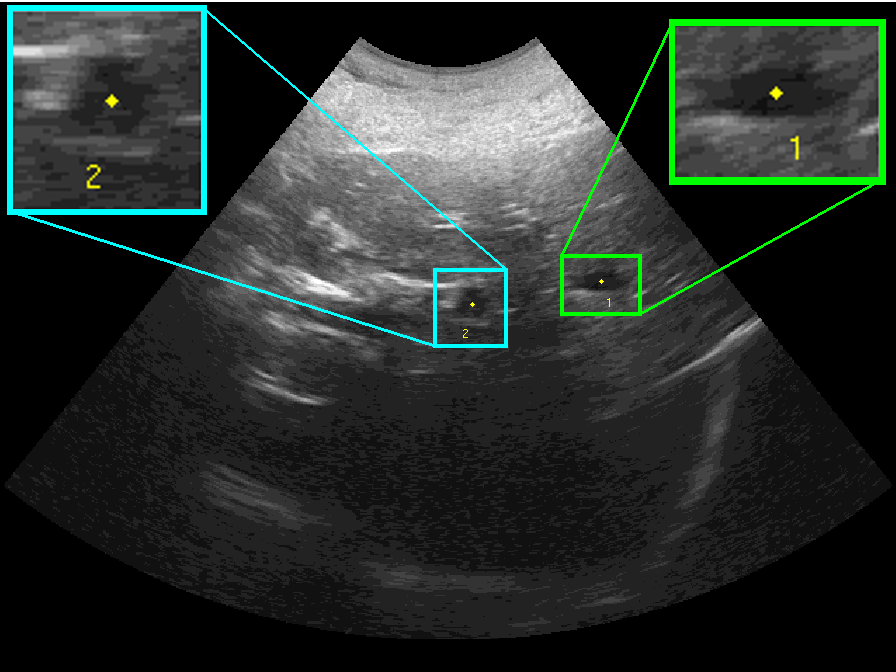
\includegraphics[width=0.5\textwidth]{figures/initialframe2}
\caption{First images in the CIL-01 sequence. The position of the each two vessels were annotated by experts in several frames.} % con anotaciones de la posicion para cada uno de los dos vasos sanguineos seleccionados
\label{fig:initialframe}
\end{figure}
For the first stage, the threshold value was experimentally defined as the intensity value that separates the $70\% $ of lower intensity pixels with $30\% $ of the most intense. For the morphological opening operation, the structuring element was established as 3x3 $pixel^2$. In the second stage, it was observed that the estimate of the centers has less noise if the region size is less than or equal to $ 1.5 $ the size of the region extracted from the first image. Finally , for the optimization, the input data were evaluated every 15s ( 3 groups of 330 samples and one of 352 ). Results of the estimation of the Centers for vessels 1 and 2, before and after optimization, are presented in Figures \ref{fig:resultados01_1} y \ref{fig:resultados02_01}, respectively. Quantitative measures of comparison between reference annotations with estimates of the method before and after optimization for the vessels 1 and 2, are presented in Tables \ref{tabla:vaso1} y \ref{tabla:vaso2}, respectively.
%Para la primera etapa, experimentalmente se definio el valor umbral como el valor de intensidad que separa el $70\%$ de los pixeles de menor intensidad con el $30\%$ de los mas intensos. 
%Para la operacion morfologica de apertura, el elemento estructurante se establecio de tamanno 3x3. 
%En la segunda etapa, se observo que la estimacion de los centros presenta menos ruido si el tamanno de las regiones seleccionadas es menor o igual que $1.5$ el tamanno de la region extraida de la primera imagen. 
%Finalmente, para la optimizacion a trozos, los datos de entrada fueron evaluados cada 15s (3 grupos de 330 muestras y uno de 352).
%Resultados de la estimacion de los centros para el vaso 1 y el vaso 2, antes y despues de la optimizacion, se presentan en las Figuras \ref{fig:resultados01_1} y \ref{fig:resultados02_01}, respectivamente. 
%
%Medidas cuantitativas de comparacion entre las anotaciones de referencia con las estimaciones del metodo antes y despues de la optimizacion, para el vaso 1 y 2, se presentan en las Tablas  \ref{tabla:vaso1} y \ref{tabla:vaso2}, respectivamente.
%
\begin{figure}[h!]
\centering
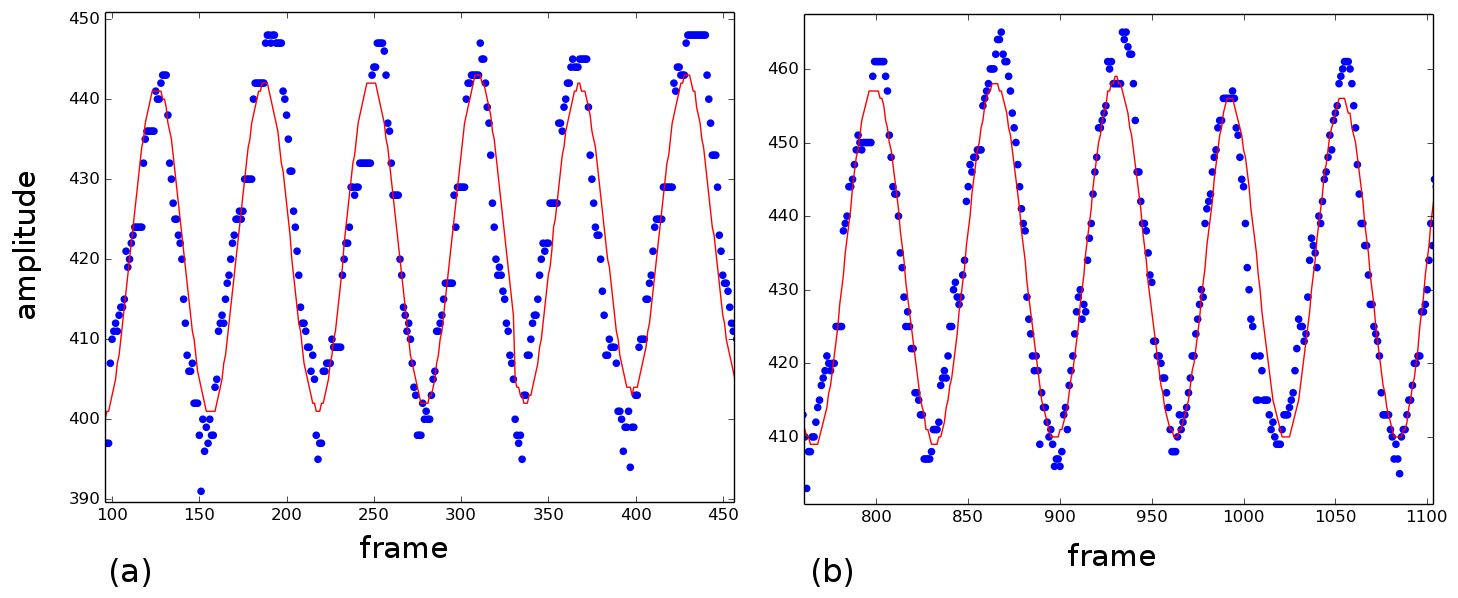
\includegraphics[width=1.0\textwidth]{figures/resultados01_1}
\caption{Tracking of $x(k)$ of vessel 1, before (blue) and after (red) the optimization process, where (a) first part of the sequence, and (b) last part of the sequence.}
\label{fig:resultados01_1}
\end{figure}
%
\begin{figure}[h!]
\centering
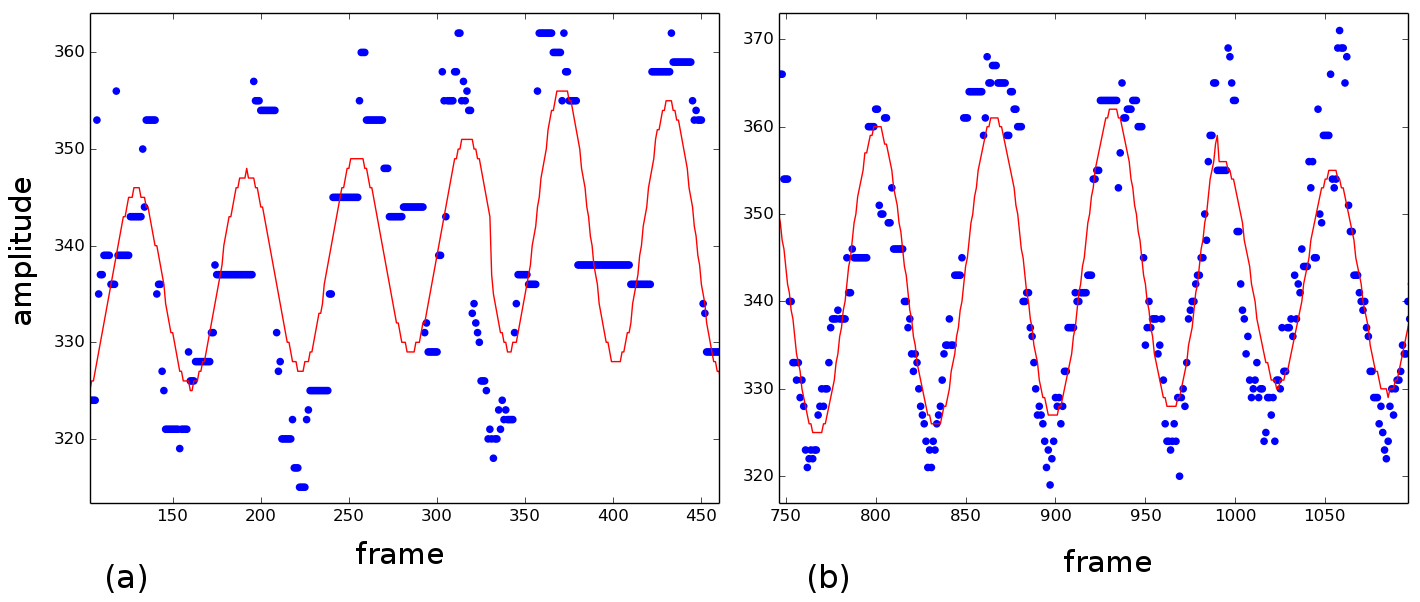
\includegraphics[width=1.0\textwidth]{figures/resultados02_1}
\caption{Tracking of $x(k)$ of vessel 2, before (blue) and after (red) the optimization process, where (a) first part of the sequence, and (b) last part of the sequence.}
\label{fig:resultados02_01}
\end{figure}
%
\begin{table}[]
\centering
\caption{Tracking results for vessel 1.}
\label{tabla:vaso1}
\begin{tabular}{lllll}
\cline{1-4}
\multicolumn{1}{|l|}{\multirow{2}{*}{\begin{tabular}[c]{@{}l@{}}Ground truth\\ CIL-01\_1.txt\end{tabular}}} & \multicolumn{3}{c|}{\textbf{Tracking error {[}mm{]}}}                                                                                 &  \\ \cline{2-4}
\multicolumn{1}{|l|}{}                                                                                      & \multicolumn{1}{c|}{\textbf{mean}} & \multicolumn{1}{c|}{\textbf{standard deviation}} & \multicolumn{1}{c|}{\textbf{95th percentile}} &  \\ \cline{1-4}
\multicolumn{1}{|l|}{\textbf{\begin{tabular}[c]{@{}l@{}}Before\\ optimization\end{tabular}}}                & \multicolumn{1}{l|}{1.049}         & \multicolumn{1}{l|}{0.651}                       & \multicolumn{1}{l|}{2.616}                    &  \\ \cline{1-4}
\multicolumn{1}{|l|}{\textbf{\begin{tabular}[c]{@{}l@{}}After\\ optimization\end{tabular}}}                 & \multicolumn{1}{l|}{1.579}         & \multicolumn{1}{l|}{0.994}                       & \multicolumn{1}{l|}{3.185}                    &  \\ \cline{1-4}
                                                                                                            &                                    &                                                  &                                               & 
\end{tabular}
\end{table}

%
\begin{table}[]
\centering
\caption{Tracking results for vessel 2.}
\label{tabla:vaso2}
\begin{tabular}{lllll}
\cline{1-4}
\multicolumn{1}{|l|}{\multirow{2}{*}{\begin{tabular}[c]{@{}l@{}}Ground truth\\ CIL-01\_2.txt\end{tabular}}} & \multicolumn{3}{c|}{\textbf{Tracking error {[}mm{]}}}                                                                                 &  \\ \cline{2-4}
\multicolumn{1}{|l|}{}                                                                                      & \multicolumn{1}{c|}{\textbf{mean}} & \multicolumn{1}{c|}{\textbf{standard deviation}} & \multicolumn{1}{c|}{\textbf{95th percentile}} &  \\ \cline{1-4}
\multicolumn{1}{|l|}{\textbf{\begin{tabular}[c]{@{}l@{}}Before\\ optimization\end{tabular}}}                & \multicolumn{1}{l|}{1.956}         & \multicolumn{1}{l|}{1.731}                       & \multicolumn{1}{l|}{5.778}                    &  \\ \cline{1-4}
\multicolumn{1}{|l|}{\textbf{\begin{tabular}[c]{@{}l@{}}After\\ optimization\end{tabular}}}                 & \multicolumn{1}{l|}{1.355}         & \multicolumn{1}{l|}{1.095}                       & \multicolumn{1}{l|}{3.394}                    &  \\ \cline{1-4}
                                                                                                            &                                    &                                                  &                                               & 
\end{tabular}
\end{table}
%
%Han sido desarrolladas pruebas preliminares en la extraccion de caracteristicas de las imagenes basados en intensidad y bordes, empleando herramientas provistas en OpenCV y Python. 
%We have developed preliminary tests for the extraction of image features based on intensity and edges, using tools provided in OpenCV and Python.


\section{Discussion}
\label{sec:discussion}



The strategy proposal seeks a first approximation of the trajectory of a point due to respiration in abdominal ultrasound sequences. It is assumed that the movement is periodic and undisturbed. The proposed method is automatic but it is not in real time. It does not require training data. The required parameters depend on the information of the first image. Therefore, it is important the good quality of  this image.
%La estrategia propuesta busca una primera aproximacion de la trayectoria que sigue un punto debido a la respiracion, en secuencias de ecografia abdominal. Se asume que el movimiento es periodico y sin perturbaciones. El metodo propuesto es automatico pero no es en tiempo real. No requiere datos de entrenamiento. Los parametros requeridos dependen de la informacion de la primera imagen. Por lo tanto, es importante que en esta imagen esten bien definidos los vasos de su entorno.

Although the evaluation is done with a single sequence, this consists of two cases , one easy ( vessel 1) and one hard (vessel 2). For the easy case, the optimization is not necessary. While for the difficult one, the optimization improves the results. The optimization gives stabilization to the system.
%Aunque la evaluacion se hace con un solo registro, este se compone de dos casos: uno facil (vaso 1) y uno dificil (vaso 2). Para el caso facil, la optimizacion resulta no ser necesaria. Mientras que para el caso dificil, la optimizacion mejora los resultados. La optimizacion le da estabilizacion al sistema.

%minimos cuadrados es facil para extraer linea base, pero para la senoidal requiere una definicion inicial de valores posibles
%MCMC no requiere la definicion de valores iniciales, pero no es algo en tiempo real

\section*{Acknowledgments}
%Este trabajo se realiza dentro del marco del trabajo de doctorado "Characterization of septal defects in three-dimensional (3D) transesophageal echocardiography (TEE)", apoyado por los profesores Sylvie Ratté y Luc Duong.
The authors thank Xavier Jordioller and Binh Tran for their suggestions and technical support.
%Los autores agradecen a Binh Tran and Xavier Jordioller por sus sugerencias y soporte tecnico.



\bibliographystyle{unsrt}
\bibliography{references/references}

\end{document}

%%%%%%%%%%%%%%%%%55
